\subsection{Unlocking the Spectrum: What Do the Axes Reveal?}

\begin{tcolorbox}[colback=gray!10, colframe=black, title=E4A02] 

Which of the following parameters does a spectrum analyzer display on the vertical and horizontal axes?
\begin{enumerate}[label=\Alph*.]
    \item Signal amplitude and time
    \item \textbf{Signal amplitude and frequency}
    \item SWR and frequency
    \item SWR and time
\end{enumerate} \end{tcolorbox}

\subsubsection{Related Concepts}

A spectrum analyzer is a crucial tool in radio communication and electronics, used for visualizing the frequency spectrum of signals. It allows engineers and technicians to see the amplitude of signals relative to frequency and helps in identifying various characteristics of electronic components and communication systems.

\subsubsection{Understanding the Axes}

The vertical axis of a spectrum analyzer typically represents the signal amplitude, often measured in decibels (dB). This provides a logarithmic scale for ease of comparison among signals of vastly different powers. 

The horizontal axis represents frequency, generally measured in hertz (Hz). This axis allows the user to identify the frequency components within a given signal, critical for analyzing modulation schemes or the frequency response of a device.

To illustrate these concepts, consider a simple representation of a spectrum analyzer output:

\begin{center}
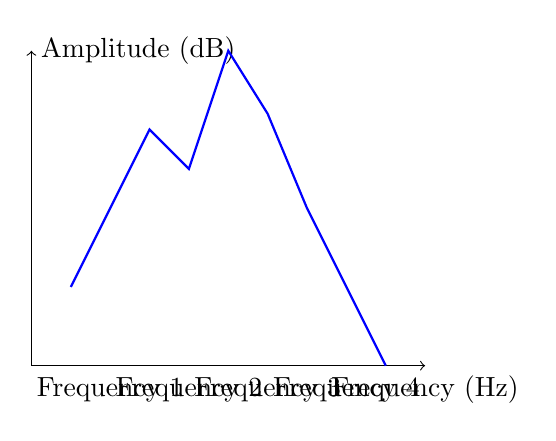
\begin{tikzpicture}
    \draw[->] (0,0) -- (0,4) node[right] {Amplitude (dB)};
    \draw[->] (0,0) -- (5,0) node[below] {Frequency (Hz)};
    
    \draw[blue, thick] plot coordinates {(0.5,1) (1,2) (1.5,3) (2,2.5) (2.5,4) (3,3.2) (3.5,2) (4,1) (4.5,0)};
    
    \node at (1,-0.3) {Frequency 1};
    \node at (2,-0.3) {Frequency 2};
    \node at (3,-0.3) {Frequency 3};
    \node at (4,-0.3) {Frequency 4};
\end{tikzpicture}
\end{center}

In this diagram, we observe peaks at various frequencies, corresponding to the amplitudes displayed on the vertical axis. 

To effectively operate a spectrum analyzer, one must be familiar with the concept of Fast Fourier Transform (FFT), as it is used to compute the spectrum of a signal. This mathematical operation converts a signal from its original domain (often time) into the frequency domain, yielding the amplitude of various frequencies that constitute the signal.

Understanding how a spectrum analyzer displays data can greatly enhance one's ability to troubleshoot and diagnose issues within radio and electronic systems.
